\documentclass{article}
\usepackage{graphicx}
\graphicspath{ {./images/} }
\usepackage[utf8x]{inputenc}
\usepackage{amsmath}
\usepackage[table]{xcolor}
\usepackage{fancyhdr}


\begin{document}
\clearpage{}
\title{FORMA \\LUCRURILOR}
\author{Chițu Raluca-Oana}
\date{}

\maketitle
\clearpage{}

\begin{abstract}

\hfill\break
\hfill\break
\hfill\break
\hfill\break
\hfill\break
\hfill\break
\hfill\break
\hfill\break
\hfill\break
\hfill\break

\textit{În ceea ce privește geometria celor vechi și algebra modernilor, dincolo de faptul că se referă la materii foarte abstracte și care nu par a fi de folos,
prima se limitează la studiul figurilor și nu poate face intelectul să lucreze fără a obosi mult imaginația}
\begin{flushright}{Marco Andreatta - Forma lucrurilor}
\end{flushright}
\end{abstract}
\hfill\break
\hfill\break
\hfill\break

\begin{center}

\includegraphics{Chimie}
\end{center}


\clearpage{}

\hfill\break
\hfill\break
\hfill\break
\hfill\break
\hfill\break
\hfill\break
\hfill\break
\hfill\break
\tableofcontents
\listoftables
\clearpage{}

\section{Introducere}

\textit{Geometrie} e un cuvânt care vine din greacă, și înseamnă ,,măsura timpului”. Termenul indică o disciplină veche, unul dintre cele mai studiate și sofisticate sisteme ale gândirii filozofice, capabil să furnizeze interpretări ale lumii în care trăim și tehnicile de care avem nevoie ca să ne putem împlini așteptările și dorințele, sistem care s-a dezvoltat printr-un proces evolutiv caracteristic speciei umane în raporturile sale cu spațiul.

\subsection{Geneza, geometria greacă}


În scrierea cuneiformă și în sistemul sexagesimal pot fi citite numerele 1,414213 și 42,42639, aproximări excelente pentru $\sqrt{2}$ și 30. $\sqrt{2}$. Reprezintă măsura diagonalelor pătratului de latură 1 și ale pătratului de latură 30, după cum se vede dintr-un calcul care necesită cunoașterea teoremei lui Pitagora - cel puțin în anumite forme particulare ei. Primii care au dezvoltat organic geometria au fost filozofii greci; ei sunt cei care au elaborat o gândire matematică dezvoltând-o din rezultate stabilite anterior, pornind de la doar puține principii de bază, oarecum evidente, pe care le-au numit \textit{axiome} sau \textit{postulate}. Thales, Democrit și Platon sunt, cu siguranță, primii gânditori pe care-i putem defini drept \textbf{idealiști}, deoarece pun la baza concepțiilor lor lumea ideilor - de la cuvântul grecesc care înseamnă \underline{,,schemă sau figură geometrică”}.

\section{Matematica lucrurilor}

Un mare matematician al Greciei antice, siracuzianul Arhimede, atacă mai direct problema. Alături de Leondardo, Galilei, Einstein, el e una dintre figurile simbol ale geniului uman;un om care a pendulat continuu între nevoia de cunoaștere și necesitatea unor soluții tehnologice pentru numeroase probleme concrete.

\subsection{Nașterea analizei matematice}

În cartea \cite {Andreatta} se vorbește despre revoluția științifică promovată de Galilei și Descartes se răspândește rapid și devine curând noua paradigmă a cercetării. Înfloresc idei noi și în alte științe, apar aplicații numeroase. Dar foarte repede devine limpede că noua metodă are nevoie de o mai mare capacitate de calcul; astfel că, după doar câteva zeci de ani, o mulțime de savanți revoluționari, printre care Christiaan Huygens, Isaac Newton, Gottfried Liebniz și mai mulți membri ai familie Bernoulli, inițiază această disciplină numită la început \textit{calculus}, cunoscută azi sub numele de \textbf{\underline {analiză matematică}}.

\clearpage{}

\subsection{Forme...mai altfel}
\hfill\break
\hfill\break
\hfill\break
\hfill\break
\begin{figure}[h]
\begin{center}
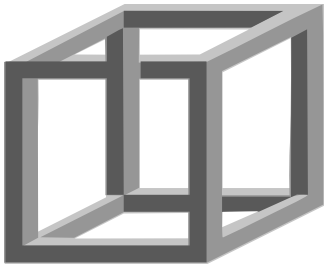
\includegraphics[width=2.5in]{Cube}
\end{center}
\caption{Cubul lui Esche}
\label{Fig.1:}
\end{figure}
\hfill\break
\hfill\break
\begin{figure}[h]
\begin{center}
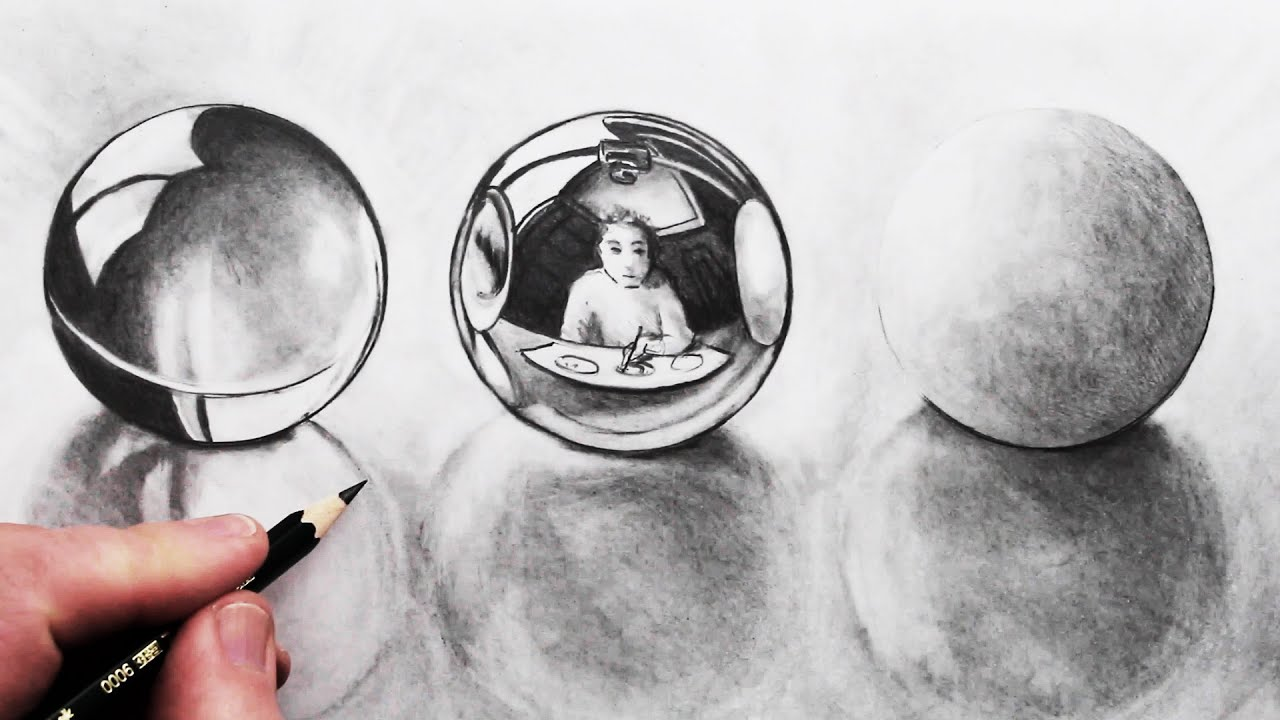
\includegraphics[width=2.8in]{Sfera}
\end{center}
\caption{Sfera}
\label{Fig.2}
\end{figure}


\clearpage{}
\subsection{Formule si tabele simpatice}
\hfill\break
\subsubsection{Formule}
\hfill\break
\hfill\break
\begin{math}
\sum_{k=2}^n = n + (n+1)^k +...+\sqrt{2}\\ 
\hfill\break
\hfill\break
\int_{a}^{b} x^2 \,dx \ 
\end{math}
\hfill\break
\begin{equation}
\label{Fractie}
 x=\sum_{n=1}^{m}  \frac{x^n}{m}
\end{equation}
\hfill\break
\hfill\break
\[ (n+1)^2 + (n+2)^3+...+y^n = z^n \]
\hfill\break
\hfill\break

\subsubsection{Tabele}
\hfill\break


\begin{table}[h!]
\centering
\begin{tabular}{||c c c ||} 
 \hline
 \textbf{FORMĂ}  & \textbf{CULOARE} & \textbf{VIZUAL} \\ 
\hline\hline
 Cub & Verde & Minge \\ 
\hline
 Triunghi & Galben & Mașină \\
\hline
\end{tabular}
\caption{Forme, culori, vizual}
\label{Tabel:1}
\end{table}
\begin{table}[h!]
\centering
\begin{tabular}{||c|| c|| c|| c||} 
 \hline
 PRODUS & QTR1(USD) & QTR2(USD) & QTR3(USD) \\ [0.5ex] 
 \hline\hline
 177 & 147 & 87837 & 787 \\ 
 \hline
 2 & 7 & 78 & 5415 \\
 \hline
 478 & 545 & 778 & 7507 \\
 \hline
 4 & 545 & 18744 & 7560 \\
 \hline
 578 & 88 & 788 & 6344 \\ [1ex] 
 \hline
\end{tabular}
\caption{Tabel cifre}
\label{table:2}
\end{table}

\clearpage{}


\section{Final}

\hfill\break
\hfill\break
\hfill\break
\hfill\break

\textit{Raporturile geometrice și figurile geometrice au fost adesea folosite în proiectele arhitecturii antice egiptene, indiene antice, grecești și romane. Catedralele medievale europene au încorporat, de asemenea, geometrie simbolică. Comunitățile spirituale indiene și himalayene au construit deseori temple și fortificații pe planurile de proiectare ale mandalei și yantrei .
Multe dintre principiile de geometrie sacră ale corpului uman și ale arhitecturii antice au fost compilate în desenul Omului Vitruvian de către Leonardo da Vinci. Ultimul desen s-a bazat el însuși pe scrierile mult mai vechi ale arhitectului roman Vitruvius}


\hfill\break
\hfill\break
\hfill\break
\hfill\break

\renewcommand\refname{Bibliografie}
\begin{thebibliography}{9}

 \bibitem{Andreatta} Marco Andreatta, \textit{Forma lucrurilor}, Ed. Humanitas, 2021.
 \bibitem{Wiki} https://ro.wikipedia.org/wiki/Geometrie

\end{thebibliography}

\hfill\break
\hfill\break
\hfill\break
\hfill\break
\hfill\break
\hfill\break
\hfill\break
\hfill\break
\hfill\break

\begin{center}
\textbf{Notă: textul utilizat a fost copiat din sursele menționate, fără prelucrare, scopul fiind doar de studiere a programului LATEX.}
\end{center}
\end{document}